%%%% APÊNDICE -- DIAGRAMAS DE BANCO DE DADOS DO NPI
%%
%% Apresenta a visão consolidada do modelo entidade-relacionamento do NPI e os
%% recortes detalhados das quatro subáreas funcionais discutidas no Capítulo
%% de Desenvolvimento. Os diagramas foram deslocados para apêndice de modo a
%% preservar a fluidez do texto principal e oferecer ao leitor interessado em
%% leitura estrutural um material consolidado.

\chapter{Diagramas de banco de dados do Nó de Pesquisa Interoperável}\label{cap:apendiceDiagramasBanco}

Este apêndice reúne, em ordem temática, os cinco diagramas entidade-relacionamento que descrevem o modelo de dados do Nó de Pesquisa Interoperável (NPI), discutidos em alto nível na Subseção~\ref{subsec:NPIDados}. Adota-se aqui o conceito de \textit{subárea} --- agrupamento lógico de entidades por afinidade funcional, tradicionalmente referido na literatura de modelagem de dados como \textit{subject area} --- para organizar a apresentação. A exposição inicia-se pela visão geral das entidades principais do banco (Seção~\ref{sec:apendiceBancoVisaoGeral}) e prossegue pelo recorte detalhado de cada uma das quatro subáreas funcionais: federação e identidade (Seção~\ref{sec:apendiceBancoFederacao}), pesquisa (Seção~\ref{sec:apendiceBancoPesquisa}), aquisição (Seção~\ref{sec:apendiceBancoAquisicao}) e vocabulário clínico (Seção~\ref{sec:apendiceBancoVocabulario}).

A separação por subárea é deliberada e reflete o agrupamento funcional adotado pelo \texttt{PrismDbContext}: a visão geral permite ao leitor observar como as principais entidades se relacionam entre si, enquanto os recortes detalhados revelam os atributos individuais, tabelas de relacionamento N:N e as cardinalidades das tabelas de junção, informação tipicamente omitida no diagrama global por uma questão de legibilidade. As entidades de catálogo SNOMED CT, em particular, materializam o uso de chaves naturais externas ao NPI, padrão decorrente da decisão arquitetural de delegar à autoridade mantenedora a unicidade global desses identificadores. Todas as demais entidades transacionais utilizam \textit{Universally Unique Identifier} (UUID) na versão~4 como chave primária, conforme detalhado no texto.

% ----------------------------------------------------------------------
\section{Visão geral das quatro subáreas funcionais}\label{sec:apendiceBancoVisaoGeral}
% ----------------------------------------------------------------------

A Figura~\ref{fig:NPIModeloDados} apresenta um diagrama entidade-relacionamento simplificado do NPI. Por concisão, foram preservados apenas os nomes da entidades e seus relacionamentos principais; os recortes individuais nas seções seguintes detalham os atributos e as cardinalidades omitidos nesta visão global.

\begin{figure}[htpb]
\captionsetup{width=0.9\textwidth}
\caption{Diagrama entidade-relacionamento simplificado do NPI.}
\label{fig:NPIModeloDados}
\centering
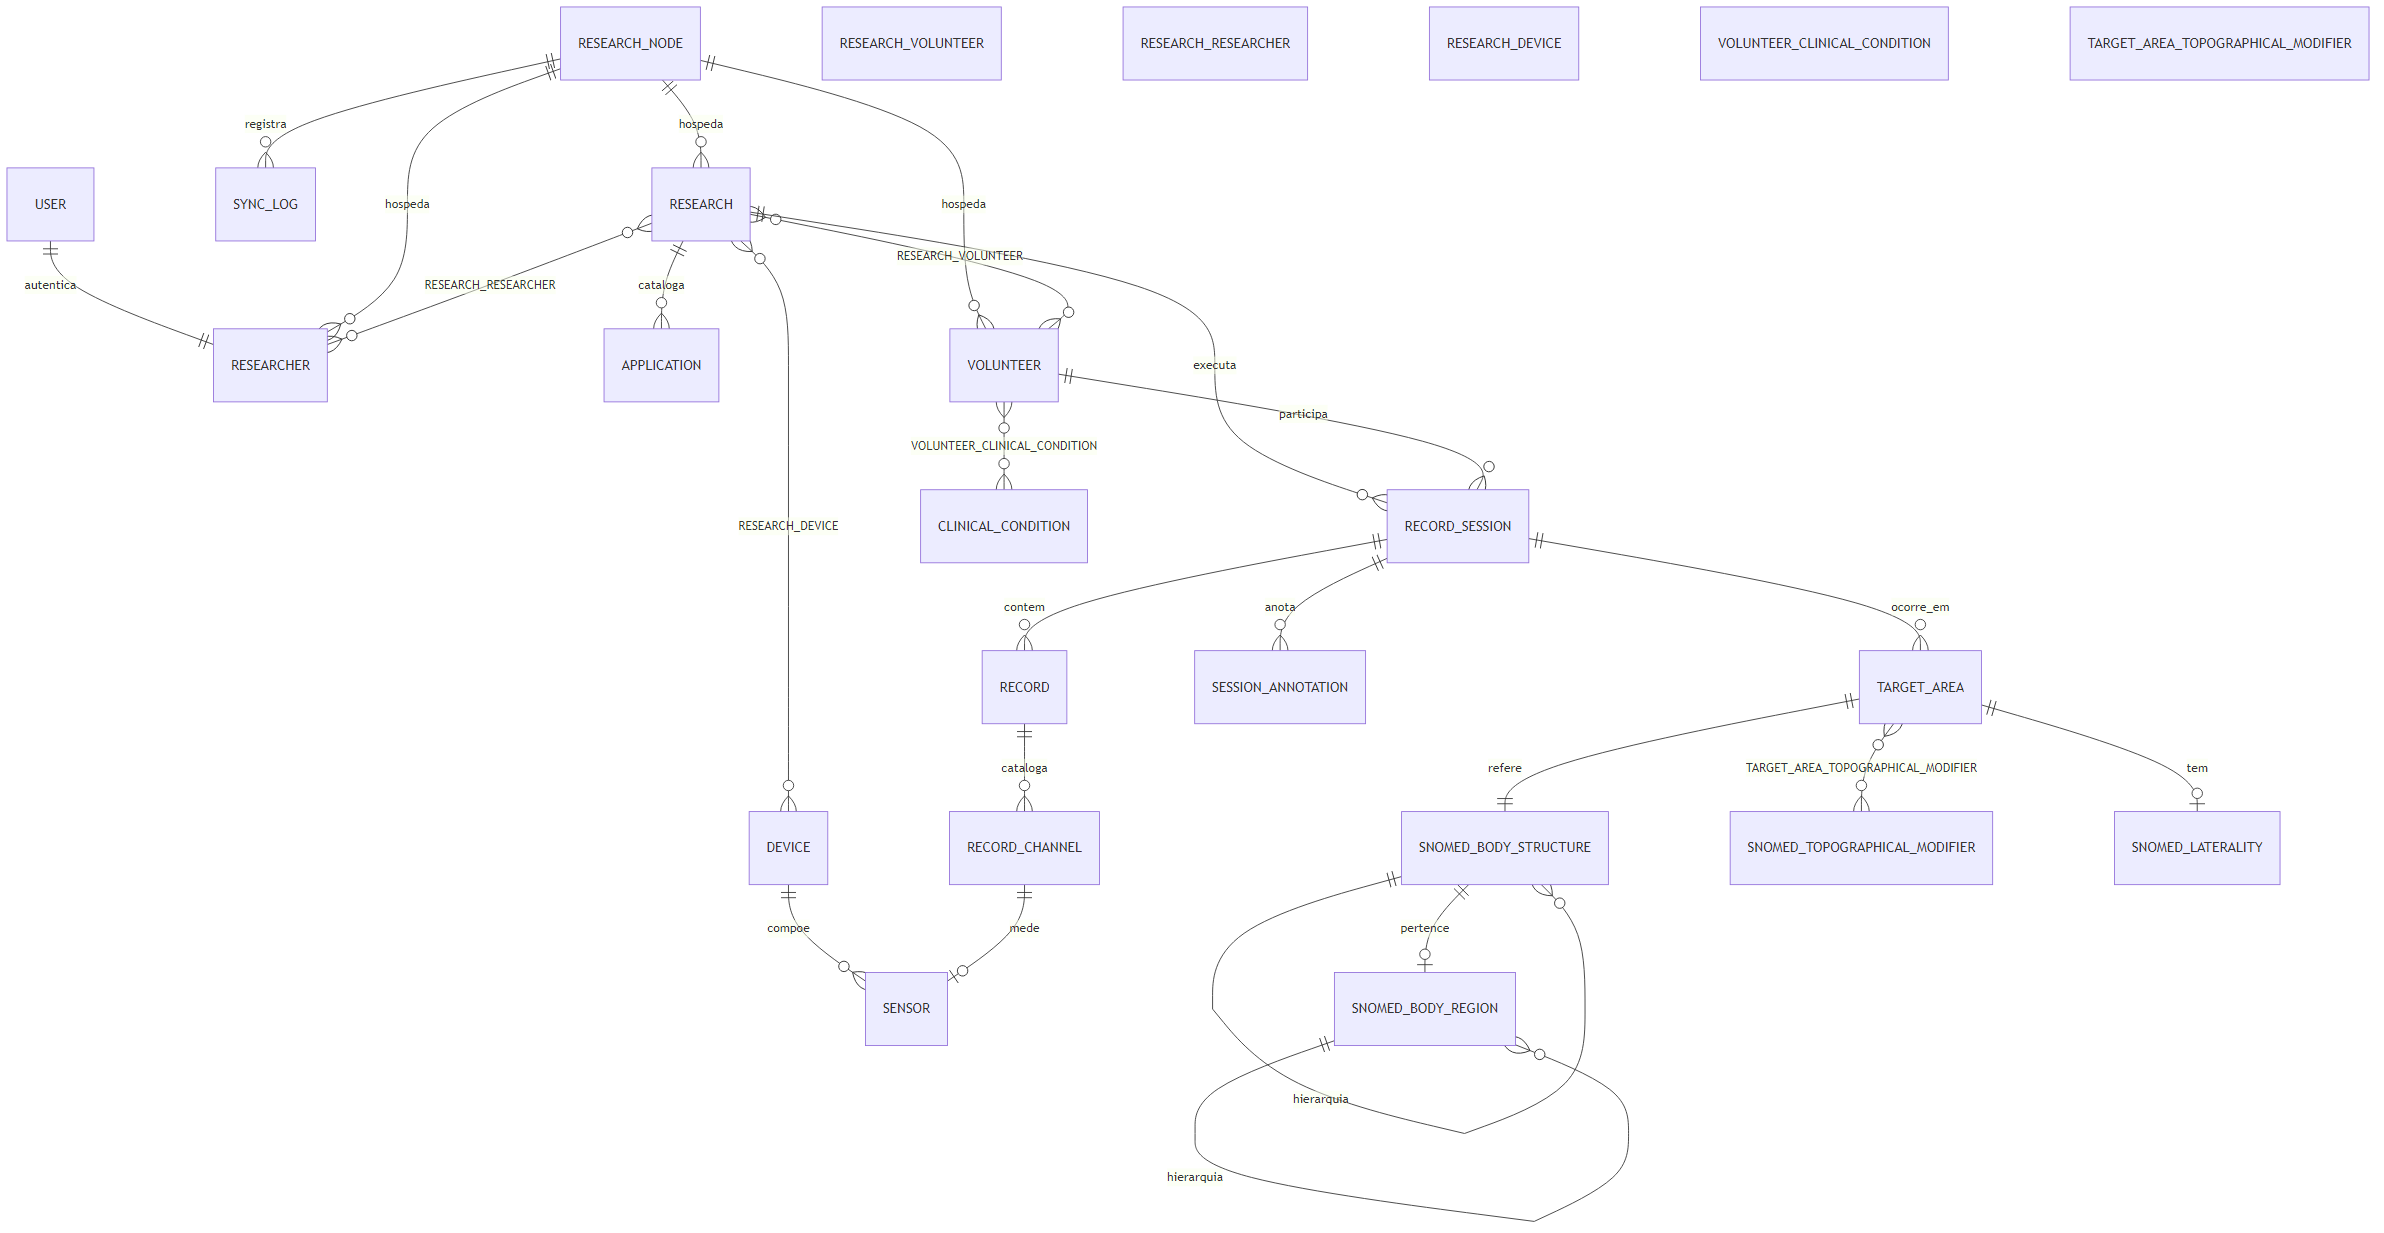
\includegraphics[scale=0.5, angle=90]{figuras/Desenvolvimento/NPI/modeloDados-visaoGeral.png}
\fonte{}
\end{figure}

% ----------------------------------------------------------------------
\section{Subárea de federação e identidade}\label{sec:apendiceBancoFederacao}
% ----------------------------------------------------------------------

A Figura~\ref{fig:NPIModeloDadosFederacao} detalha as entidades responsáveis pela operação multinó. A entidade \texttt{ResearchNode} representa cada nó da rede, tanto outros NPIs quanto aplicações de pesquisas conectadas a esse nó, armazena seu certificado X.509 e mantém o atributo \texttt{CertificateFingerprint} (resumo SHA-256 do certificado) declarado como índice único, configurando a chave natural pela qual nós se reconhecem mutuamente durante o \textit{handshake}. As entidades \texttt{User} e \texttt{Researcher} modelam os agentes humanos com acesso ao nó. A entidade \texttt{SyncLog} mantém o histórico de cada sincronização realizada com nós remotos --- \textit{status}, marcas temporais, contadores em formato JSON e mensagens de erro --- e serve de base à estratégia de sincronização incremental discutida na Subseção~\ref{subsec:NPITrocaDados}.

\begin{figure}[htpb]
\captionsetup{width=0.9\textwidth}
\caption{Subárea de \textbf{federação e identidade}: atributos detalhados das entidades responsáveis pela operação multinó (\texttt{ResearchNode}, \texttt{User}, \texttt{Researcher}, \texttt{Application}, \texttt{SyncLog}).}
\label{fig:NPIModeloDadosFederacao}
\centering
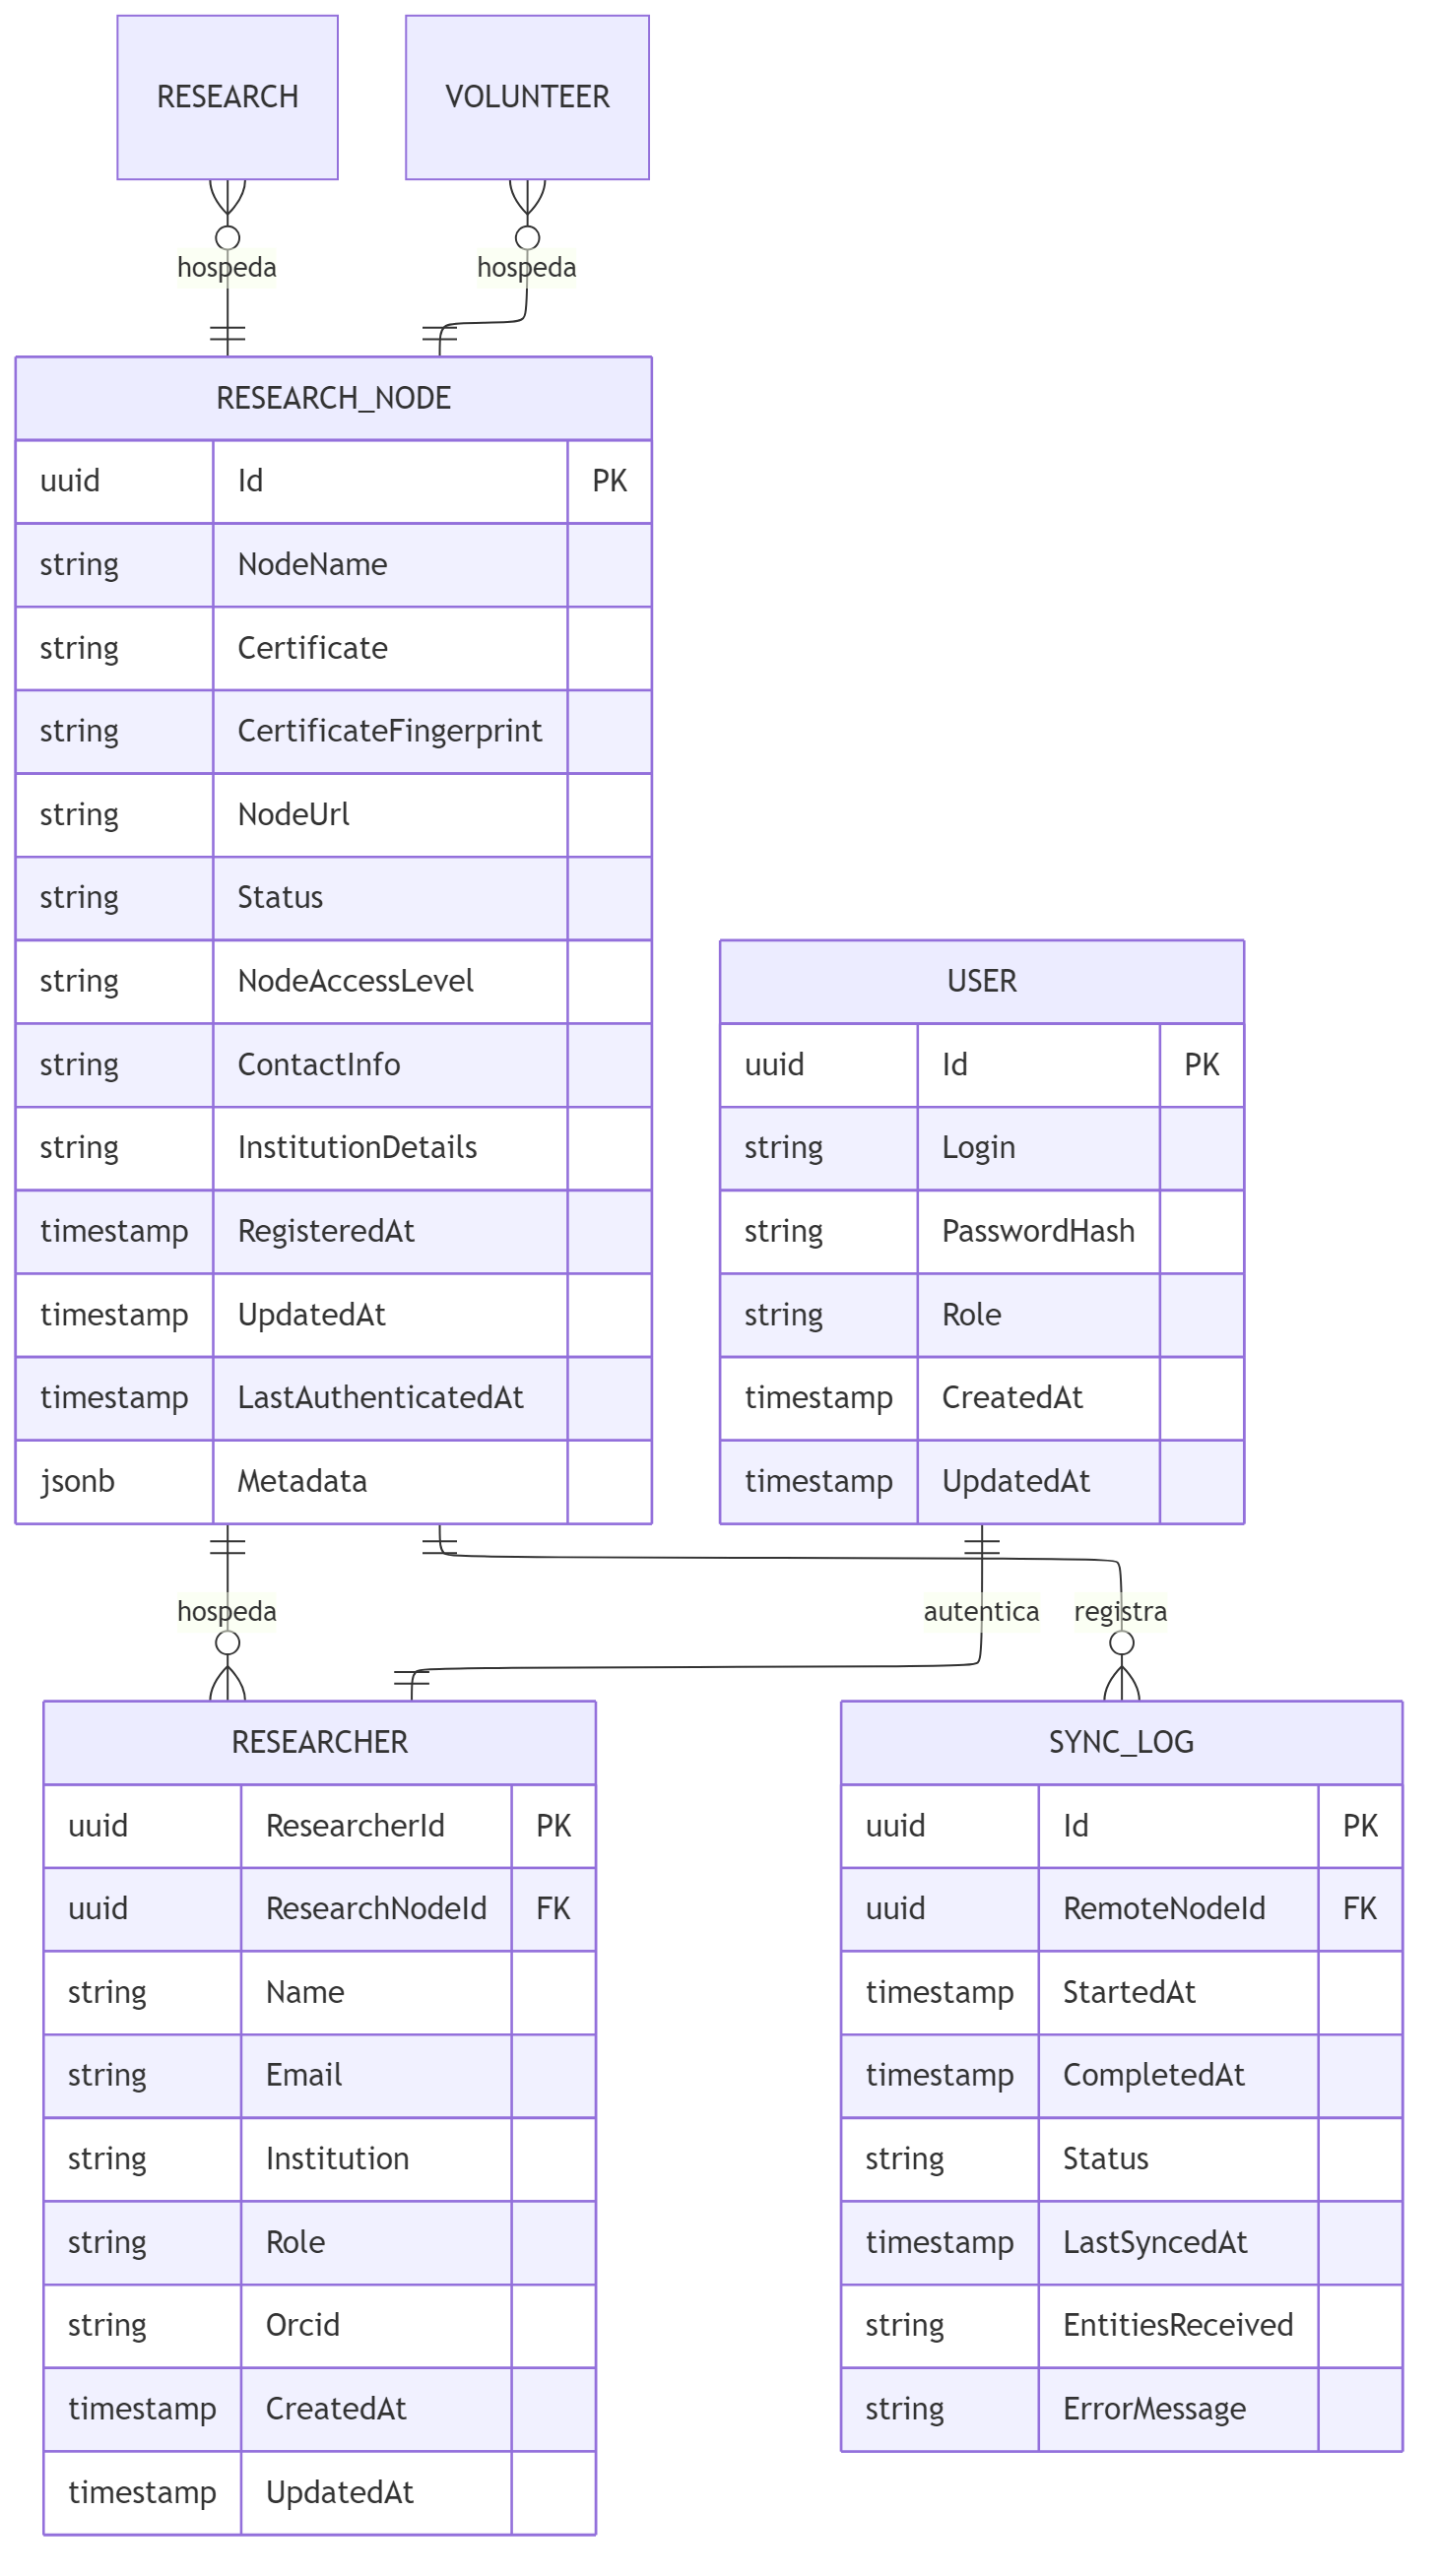
\includegraphics[width=0.9\textwidth]{figuras/Desenvolvimento/NPI/modeloDados-familia-federacao.png}
\fonte{}
\end{figure}

% ----------------------------------------------------------------------
\section{Subárea de pesquisa}\label{sec:apendiceBancoPesquisa}
% ----------------------------------------------------------------------

A subárea de pesquisa é organizada em torno da entidade \texttt{Research} e foi dividida em dois recortes complementares por questão de legibilidade: o primeiro (Figura~\ref{fig:NPIModeloDadosPesquisaProjeto}) reúne o projeto, a equipe de pesquisadores e a instrumentação utilizada; o segundo (Figura~\ref{fig:NPIModeloDadosPesquisaVoluntario}) detalha os voluntários e suas condições clínicas. A modelagem por tabelas de junção é comum aos dois recortes: as tabelas materializam relações N:N e carregam atributos de contexto --- por exemplo, o papel do pesquisador no projeto ou o \textit{status} de inscrição do voluntário --- que não pertencem nem à entidade-mãe nem à entidade vinculada. Essa estrutura permite que um mesmo voluntário participe simultaneamente de mais de um projeto sob papéis distintos sem duplicação de cadastro.

A Figura~\ref{fig:NPIModeloDadosPesquisaProjeto} apresenta o recorte de projeto, equipe e instrumentação. A entidade \texttt{Research} agrega relacionamentos N:N com pesquisadores (\texttt{Researcher}), por meio de \texttt{ResearchResearcher}, e com dispositivos (\texttt{Device}), por meio de \texttt{ResearchDevice}; cada dispositivo, por sua vez, compõe-se de um ou mais \texttt{Sensor}. As tabelas de junção registram, respectivamente, a designação de pesquisador principal e o estado de calibração do dispositivo no contexto do projeto.

\begin{figure}[htpb]
\captionsetup{width=0.9\textwidth}
\caption{Subárea de \textbf{pesquisa} (recorte de projeto, equipe e instrumentação): entidades \texttt{Research}, \texttt{Researcher}, \texttt{Device} e \texttt{Sensor}, com as tabelas de junção \texttt{ResearchResearcher} e \texttt{ResearchDevice}.}
\label{fig:NPIModeloDadosPesquisaProjeto}
\centering
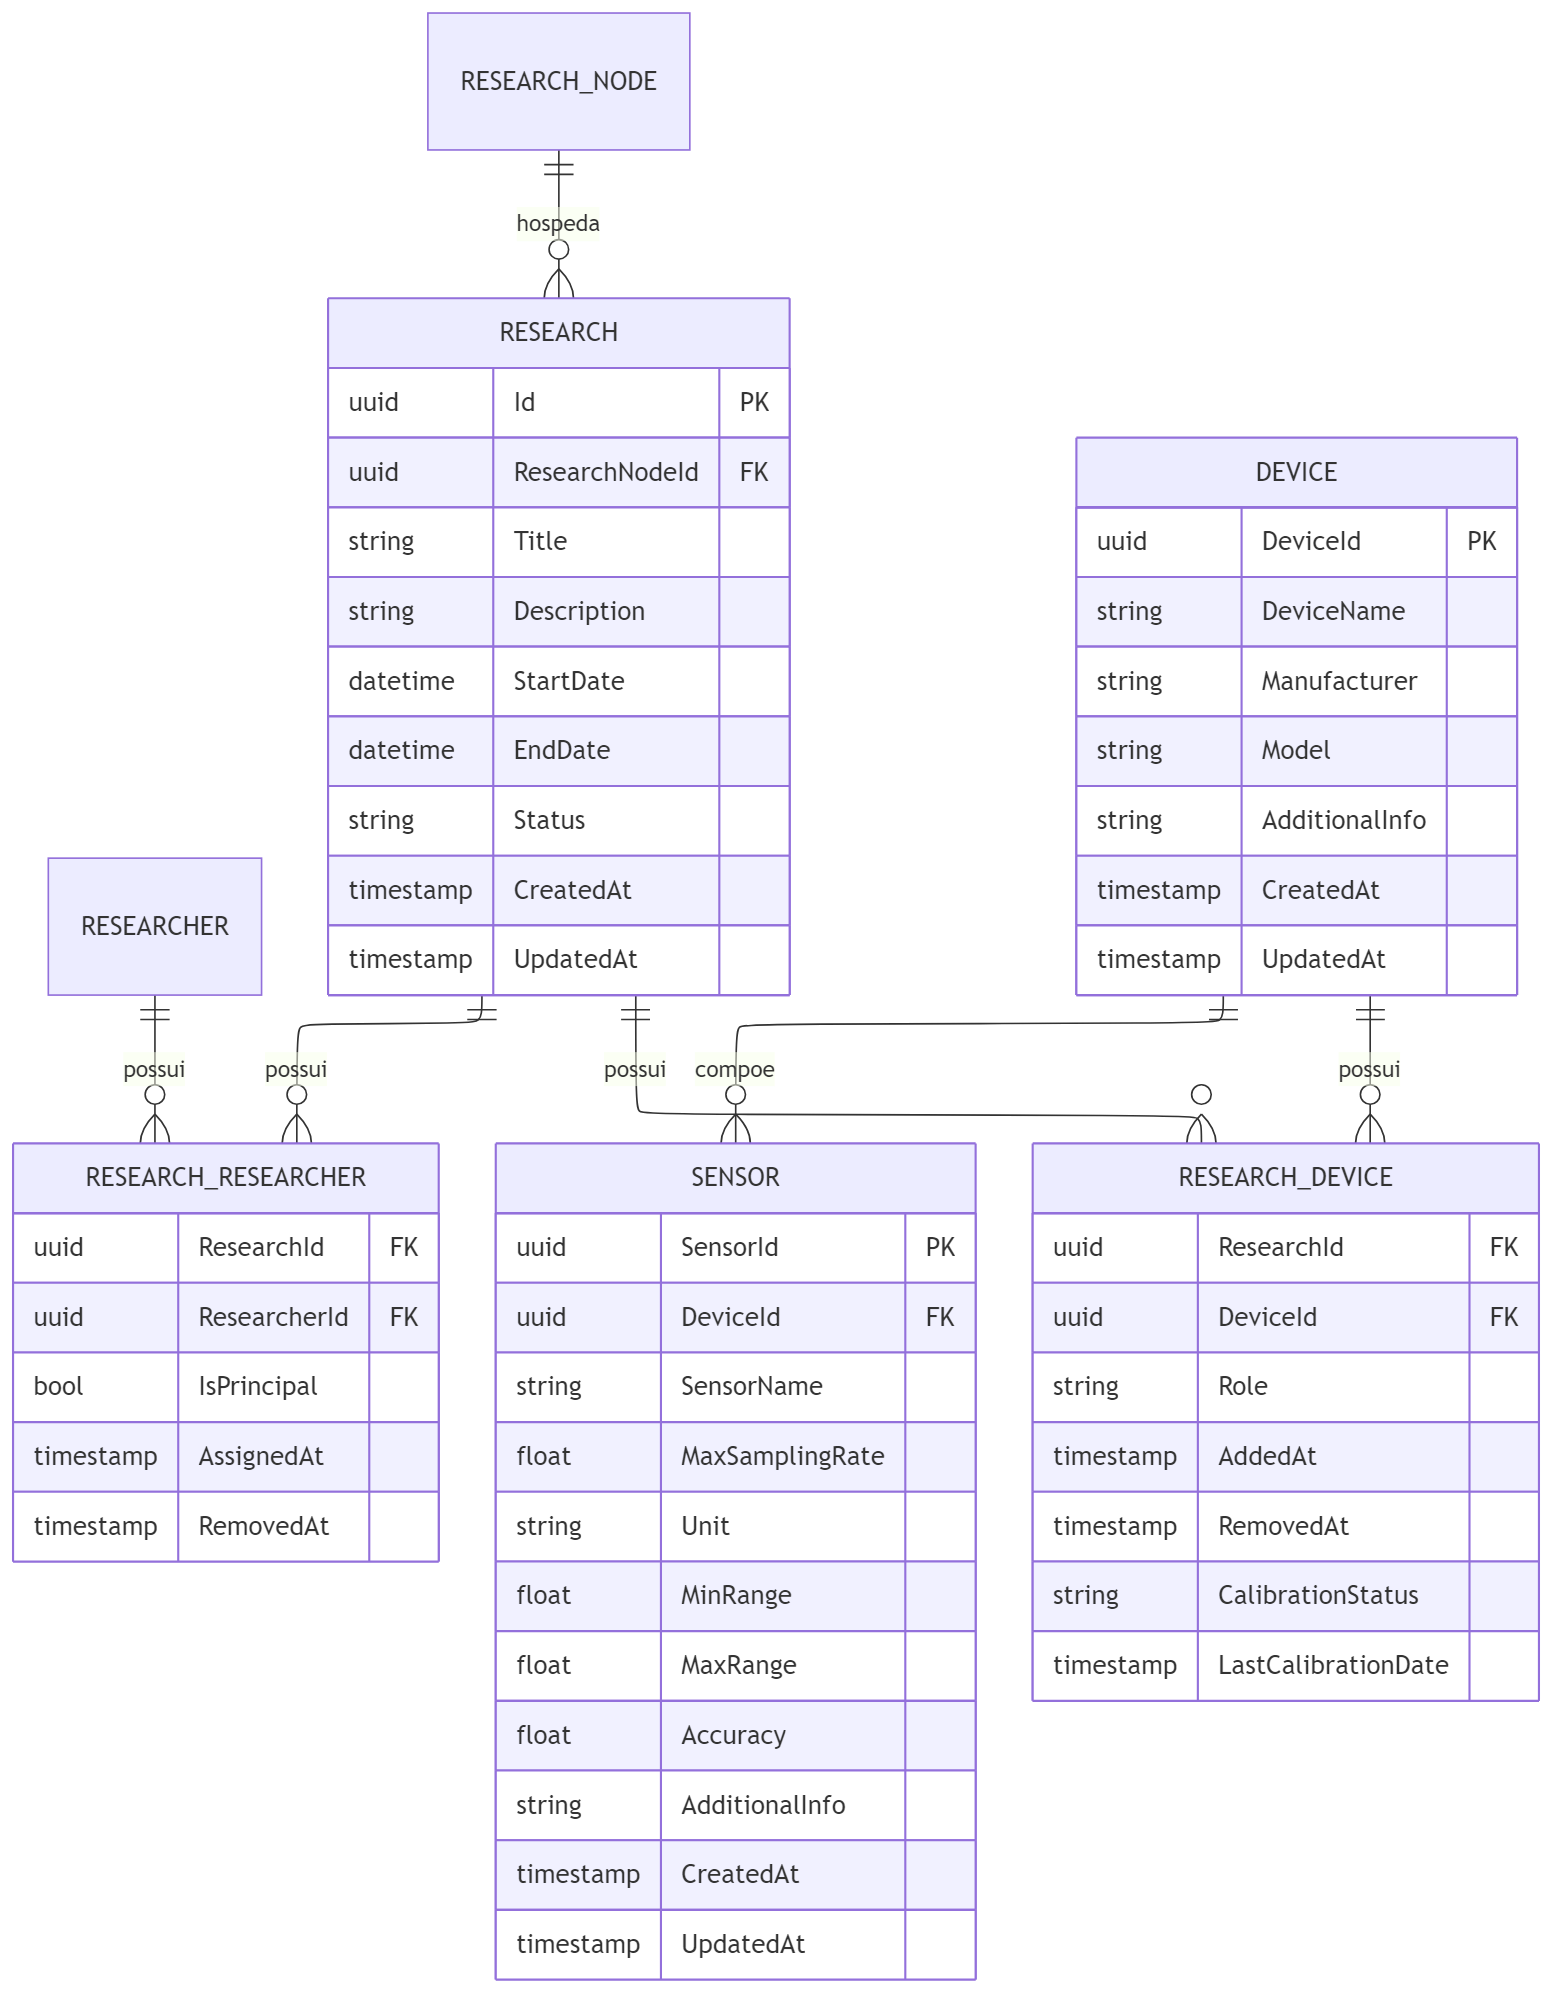
\includegraphics[width=0.9\textwidth]{figuras/Desenvolvimento/NPI/modeloDados-familia-pesquisa-projeto.png}
\fonte{}
\end{figure}

A Figura~\ref{fig:NPIModeloDadosPesquisaVoluntario} apresenta o recorte de voluntários e dados clínicos. A entidade \texttt{Volunteer} relaciona-se ao projeto por \texttt{ResearchVolunteer} --- que mantém o \textit{status} de inscrição, a versão do termo de consentimento assinado e, eventualmente, a justificativa de exclusão --- e ao vocabulário clínico por \texttt{VolunteerClinicalCondition}, junção que vincula cada voluntário às condições registradas no catálogo SNOMED CT detalhado na Seção~\ref{sec:apendiceBancoVocabulario}.

\begin{figure}[htpb]
\captionsetup{width=0.9\textwidth}
\caption{Subárea de \textbf{pesquisa} (recorte de voluntários e dados clínicos): entidades \texttt{Volunteer} e \texttt{ClinicalCondition}, com as tabelas de junção \texttt{ResearchVolunteer} e \texttt{VolunteerClinicalCondition}.}
\label{fig:NPIModeloDadosPesquisaVoluntario}
\centering
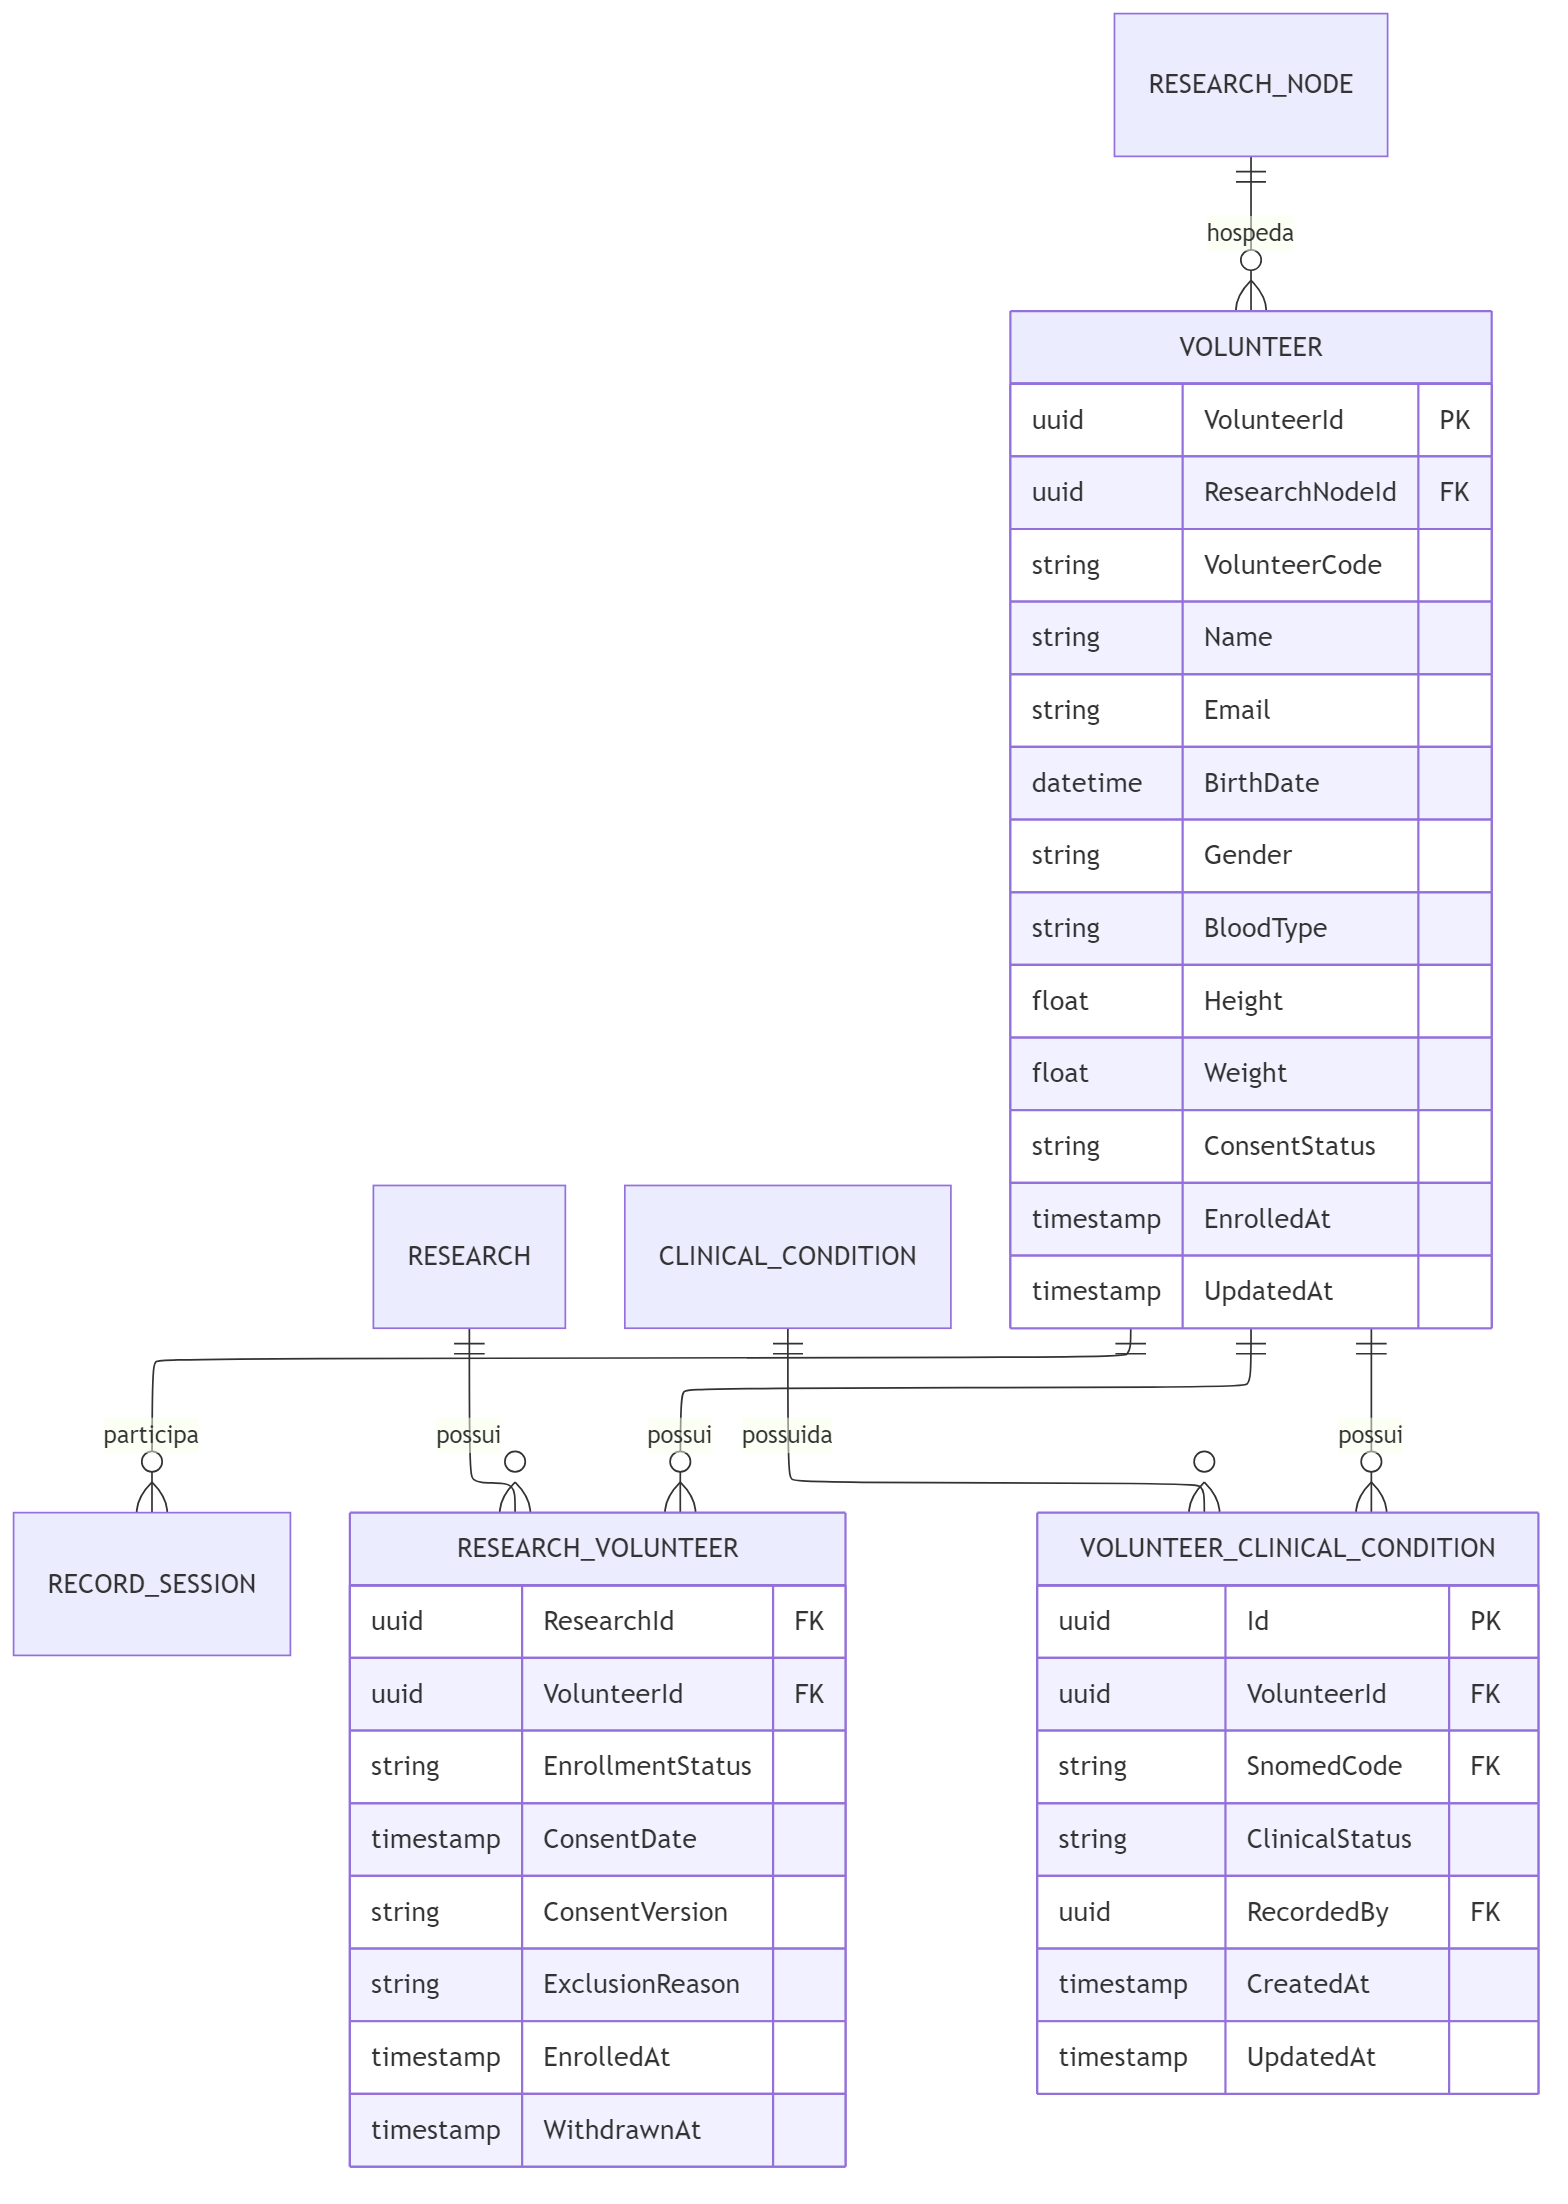
\includegraphics[width=0.9\textwidth]{figuras/Desenvolvimento/NPI/modeloDados-familia-pesquisa-voluntario.png}
\fonte{}
\end{figure}

% ----------------------------------------------------------------------
\section{Subárea de aquisição}\label{sec:apendiceBancoAquisicao}
% ----------------------------------------------------------------------

A Figura~\ref{fig:NPIModeloDadosAquisicao} detalha o ciclo da coleta. A entidade \texttt{RecordSession} representa uma sessão de coleta vinculada a um voluntário e a uma pesquisa; \texttt{Record} agrega os registros gerados em cada sessão; \texttt{RecordChannel} corresponde a um canal individual de sinal, com sua taxa de amostragem, contagem de amostras e referência à URI do \textit{blob} bruto armazenado no Azure Blob Storage. A entidade \texttt{TargetArea} interliga as sessões de aquisição ao vocabulário clínico, registrando, para cada sessão, a região anatômica alvo da medição e os modificadores aplicáveis; anotações descritivas livres ficam em \texttt{SessionAnnotation}. O atributo \texttt{UpdatedAt} de \texttt{RecordChannel} é o \textit{watermark} consultado pelo protocolo de sincronização incremental (Subseção~\ref{subsec:NPITrocaDados}) para identificar as alterações posteriores ao último ponto de corte conhecido pelo nó consumidor.

\begin{figure}[htpb]
\captionsetup{width=0.9\textwidth}
\caption{Subárea de \textbf{aquisição}: ciclo da coleta modelado por \texttt{RecordSession}, \texttt{Record}, \texttt{RecordChannel}, \texttt{TargetArea} e \texttt{SessionAnnotation}.}
\label{fig:NPIModeloDadosAquisicao}
\centering
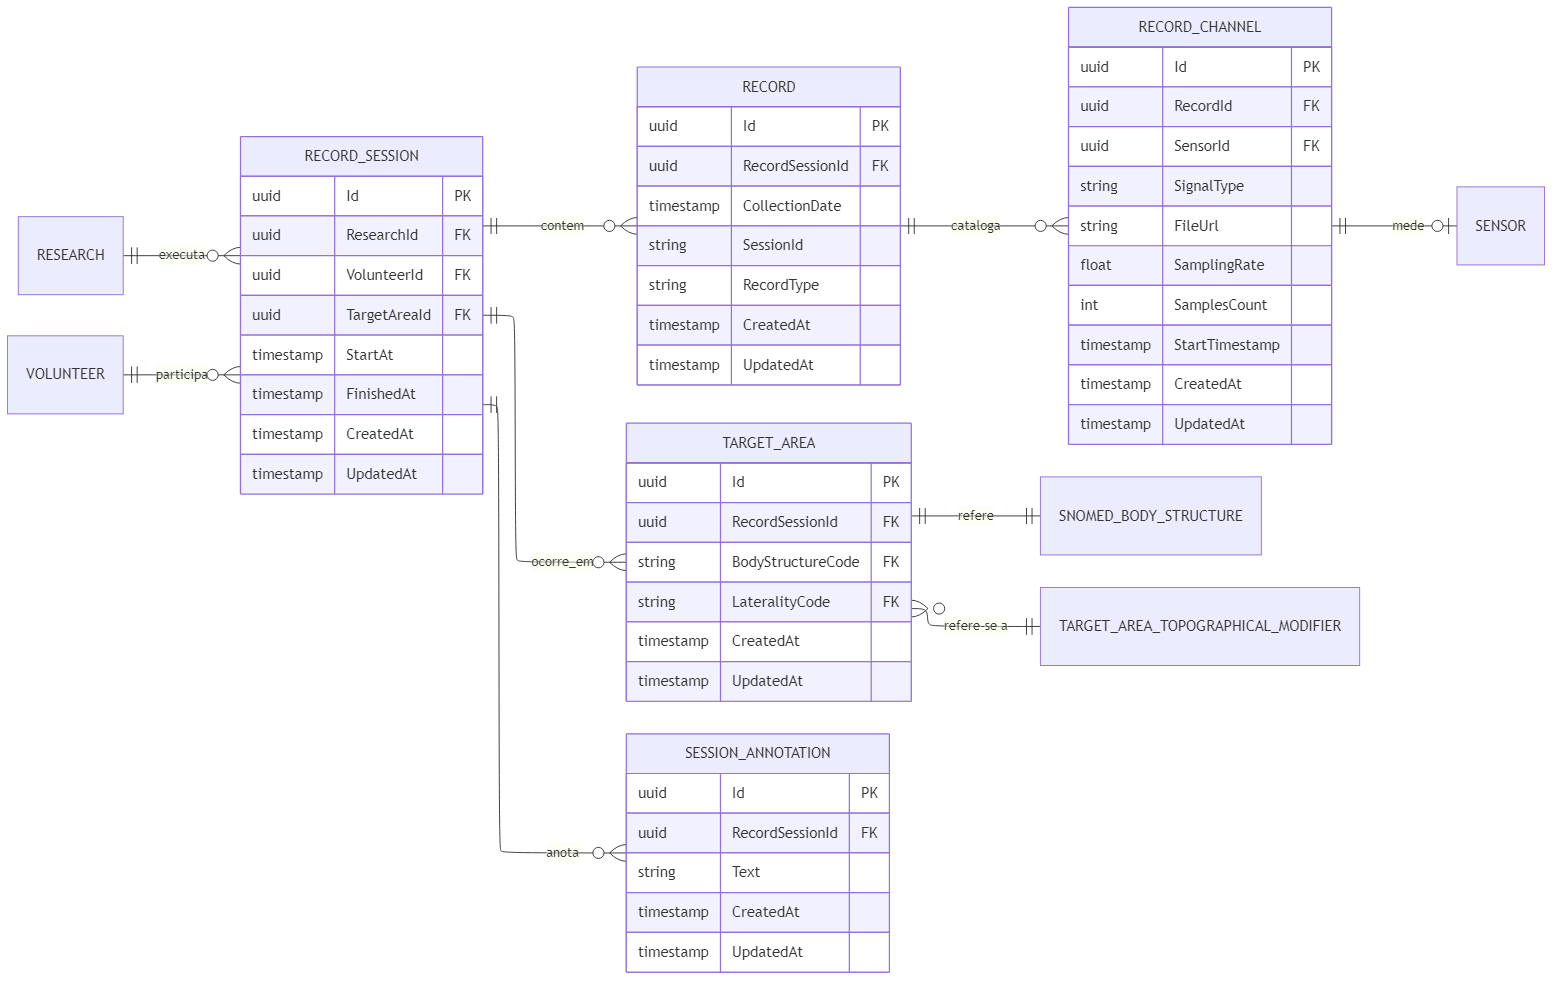
\includegraphics[width=0.9\textwidth]{figuras/Desenvolvimento/NPI/modeloDados-familia-aquisicao.png}
\fonte{}
\end{figure}

% ----------------------------------------------------------------------
\section{Subárea de vocabulário clínico}\label{sec:apendiceBancoVocabulario}
% ----------------------------------------------------------------------

A Figura~\ref{fig:NPIModeloDadosVocabulario} detalha as entidades de vocabulário clínico mapeadas à terminologia SNOMED CT: estruturas anatômicas (\texttt{SnomedBodyStructure}), regiões corporais (\texttt{SnomedBodyRegion}), modificadores topográficos (\texttt{SnomedTopographicalModifier}) e a entidade \texttt{ClinicalCondition}. As tabelas de junção que vinculam essas entidades a voluntários e a áreas-alvo materializam a contextualização semântica do biossinal: cada \texttt{RecordChannel} aponta para uma \texttt{TargetArea}, que por sua vez referencia uma estrutura anatômica, uma lateralidade e zero ou mais modificadores topográficos. A escolha do código SNOMED como chave natural global elimina a possibilidade de colisão semântica entre nós: dois NPIs que carreguem a mesma estrutura corporal o farão com o mesmo \texttt{SnomedCode}, ainda que tenham importado a partir de fontes distintas, sustentando a estratégia de \textit{last-write-wins} por \textit{watermark} \texttt{UpdatedAt} adotada pelo protocolo de sincronização (Subseção~\ref{subsec:NPITrocaDados}).

\begin{figure}[htpb]
\captionsetup{width=0.9\textwidth}
\caption{Subárea de \textbf{vocabulário clínico}: entidades SNOMED CT (estruturas anatômicas, regiões corporais, modificadores topográficos e lateralidade) e \texttt{ClinicalCondition}, com as junções para voluntários e áreas-alvo.}
\label{fig:NPIModeloDadosVocabulario}
\centering
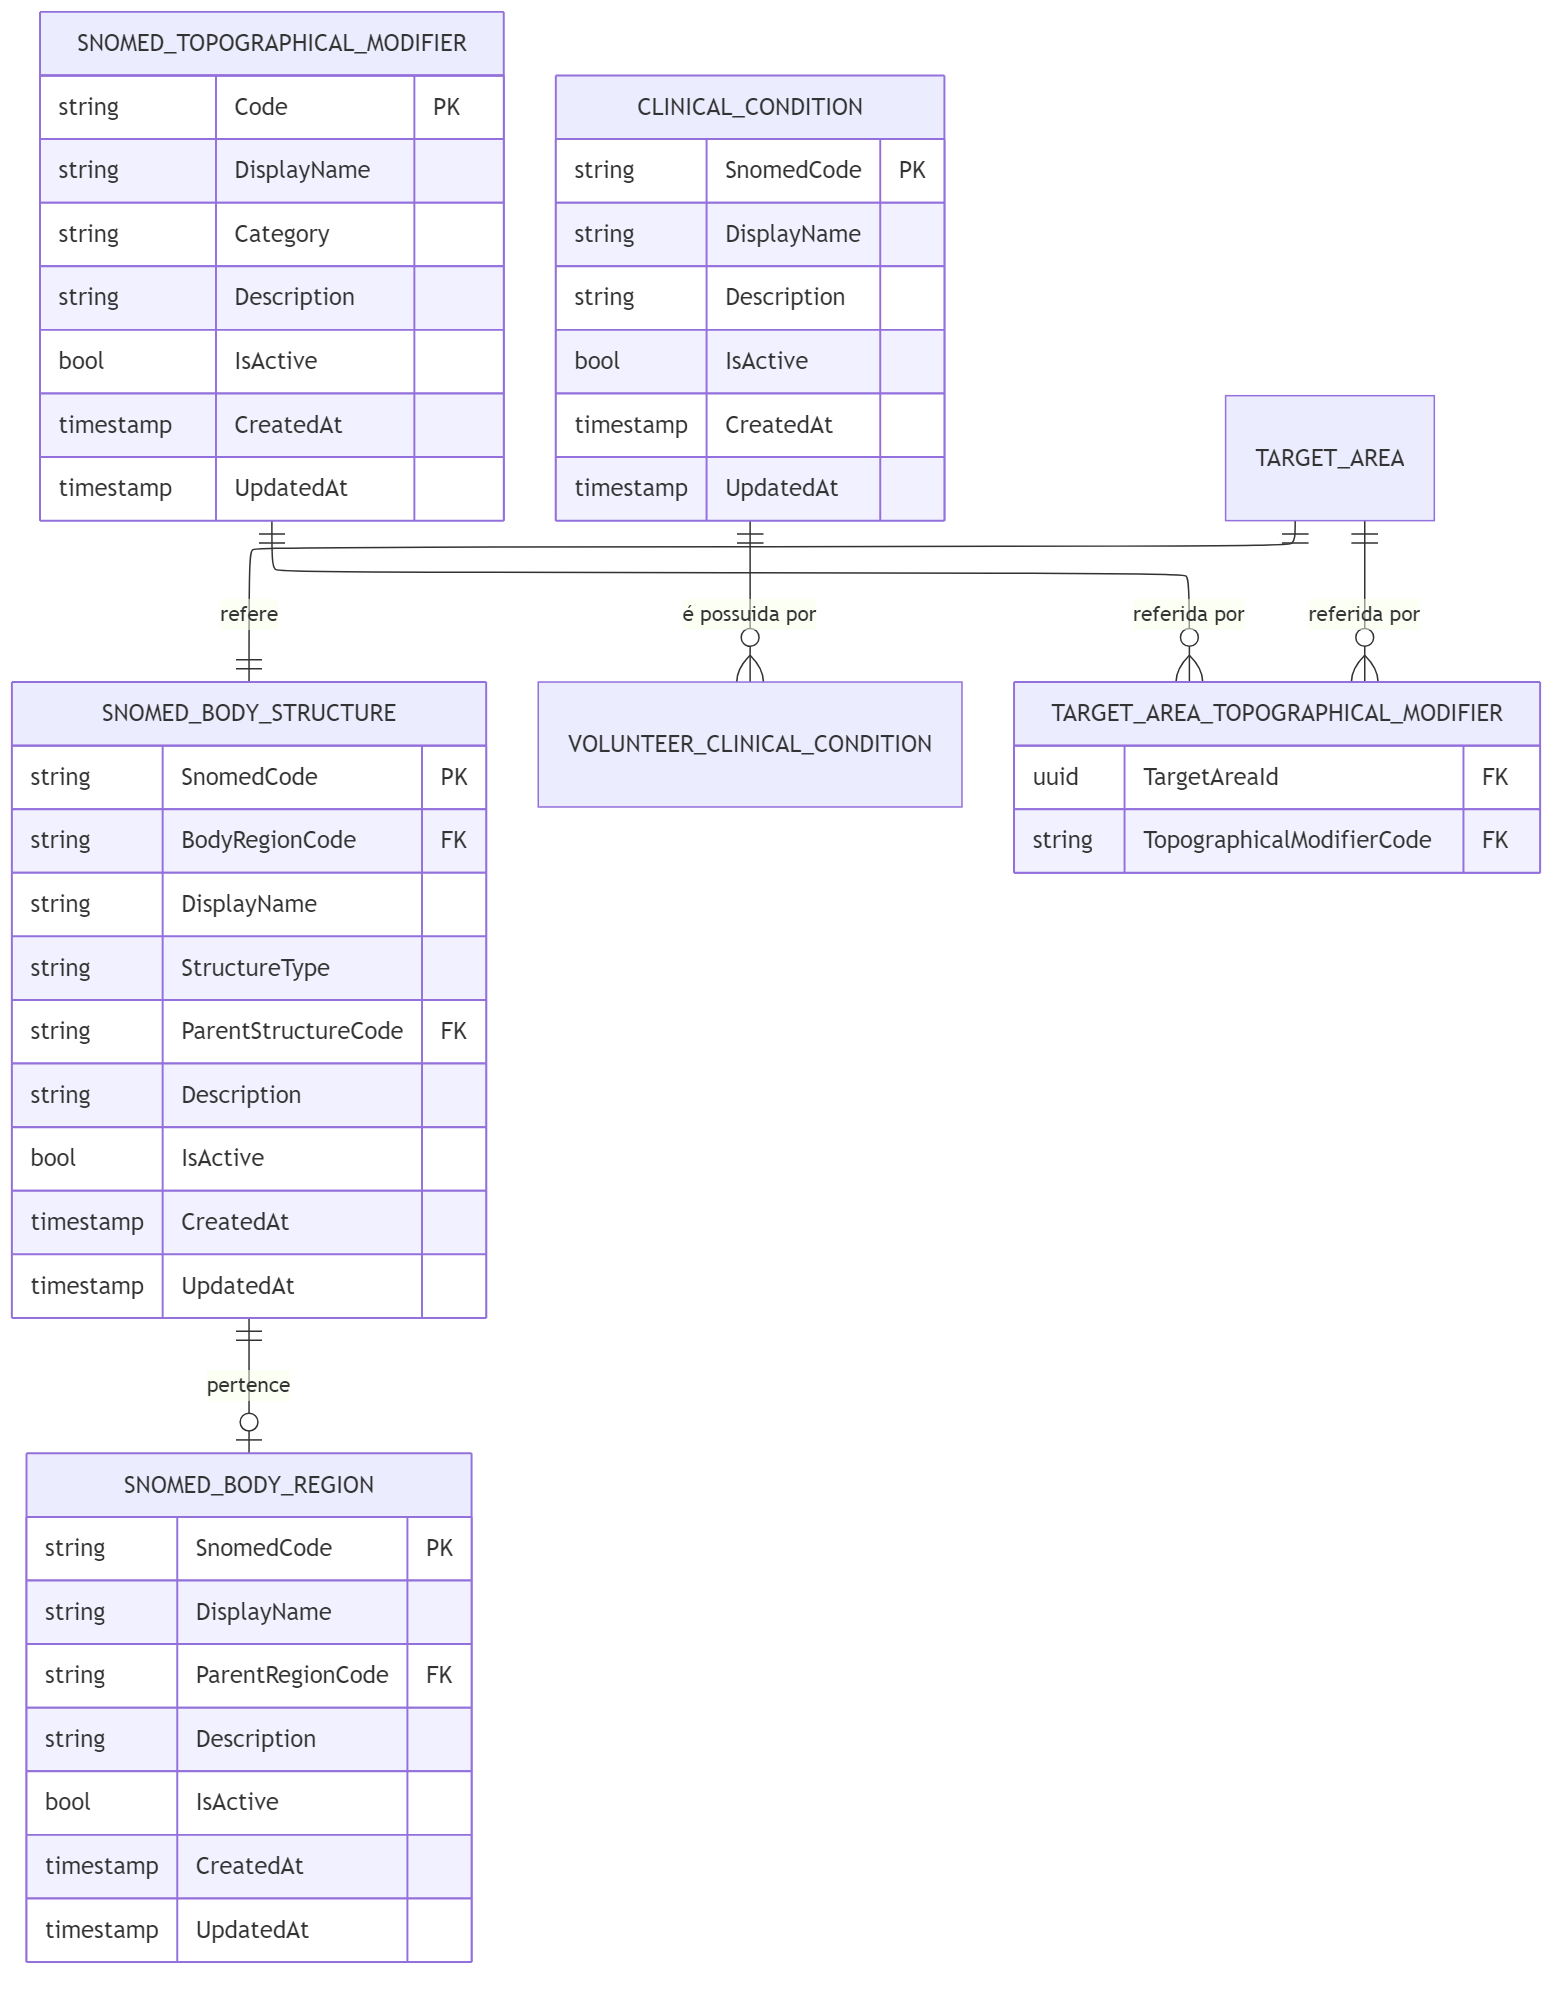
\includegraphics[width=0.9\textwidth]{figuras/Desenvolvimento/NPI/modeloDados-familia-vocabulario.png}
\fonte{}
\end{figure}
